\documentclass[SE,authoryear,toc]{article}
%\input{meta}

% Package imports go here.

\usepackage{graphicx}
\usepackage{caption}
\usepackage{subcaption}

% Local commands go here.
\newcommand{mcat}{m_{\mathrm{cat}}}
\newcommand{mtrue}{m_{\mathrm{true}}}
\newcommand{deltam}{\delta_m}
\newcommand{Deltam}{\Delta\,m}

%If you want glossaries
%\input{aglossary.tex}
%\makeglossaries

\title{Rubin Baseline Calibration Plan}

% Optional subtitle
% \setDocSubtitle{A subtitle}

\author{%
Parker Fagrelius, Eli Rykoff
}

% \setDocRef{SITCOMTN-086}
% \setDocUpstreamLocation{\url{https://github.com/lsst-sitcom/sitcomtn-086}}

\date{\vcsDate}

% Optional: name of the document's curator
% \setDocCurator{The Curator of this Document}

% \setDocAbstract{
% Current baseline plan for the year 1 minimum viable product as delivered for ORR.
% }

% Change history defined here.
% Order: oldest first.
% Fields: VERSION, DATE, DESCRIPTION, OWNER NAME.
% See LPM-51 for version number policy.
% \setDocChangeRecord{
%   \addtohist{1}{YYYY-MM-DD}{Unreleased.}{Parker Fagrelius}
% }


\begin{document}

% Create the title page.
\maketitle
% Frequently for a technote we do not want a title page  uncomment this to remove the title page and changelog.
% use \mkshorttitle to remove the extra pages


\appendix

\section{Introduction}

The basic question of photometric calibration of an astronomical survey is how
to take raw counts output from the camera (in arbitrary Analog-Digital Units
(ADU)) and convert these to calibrated fluxes in nanoJansky (nJy).  In order
for this procedure to yield uniform results across the camera and the sky, it
must take into account variations that are both achromatic (``gray'') and
chromatic, that latter of which depend on the spectral energy distribution (SED) of each
object.  This includes variations in the atmosphere as a function of time and
airmass; spatial variations in the filter and detectors; pixel size variations;
and various sensor effects such as charge transfer ineffeciency (CTI) and the
Brighter Fatter Effect (BFE).

This technote describes the baseline photometric calibration plan for Rubin
Commissioning and the first year of data release production for the LSST
Survey.  This includes plans on performing instrumental signature reduction
(ISR), which is also known as ``detrending''; correct flat-fielding;
background/foreground subtraction; and derivation of a uniform photometric
calibration over the full survey.  It also includes plans for generating
``calibration frames'' such as bias, darks, and various types of flats,
incorporating LEDs, a class 4 tunable laser, and a novel Collimated Beam
Projector (CBP).  We expect that this is not the final calibration plan for the
LSST survey, but rather a first minimal viable product suitable for the first
year of survey observations to meet our required goals for repeatability and
uniformity.  Further improvements are planned to incorporate more effects,
although our plan is to take as much calibration data early on to be able to
reprocess early data with improved algorithms.

The calibration plan in this technote is heavily influenced by the Dark Energy
Survey, which achieved better than $2~\mathrm{mmag}$ uniformity over
$5000\,\mathrm{deg}^2$ in the Southern sky~(Rykoff et al. 2023).  In
particular, we refer the reader to Bernstein et al. 2017 (henceforth B17) and
Burke, Rykoff, et al. 2018 (henceforth BR18).

\section{Requirements}
The requirements on calibration are defined in the Science Requirements Document (LPM-17). The photometric quality and accuracy of the LSST data products is driven by four main components:
\begin{enumerate}
    \item Relative photometry (repeatability)
    \item Stability across the sky (spatial uniformity)
    \item Relative accuracy (color zero-points)
    \item Transfer to physical flux scale (external absolute photometry)
\end{enumerate}

The requirements for photometric calibration accuracy are specified using the following error decomposition (valid in the limit of small errors):
\begin{equation}
    \mcat = mtrue +\sigma+\deltam (x,y,\theta,\alpha,\delta,\mathrm{SED},t)+\Deltam
\end{equation}
where $\mtrue$ is the true magnitude defined by eqs. 4 and 7, $\mcat$ is the cataloged LSST magnitude, $\sigma$ is the random photometric error (including random calibration errors and count extraction errors), and $\Deltam$ is the overall (constant) offset of the internal survey system from a perfect AB system (the six values of $\Deltam} are equal for all the cataloged objects).
Here, $\deltam$ describes the various systematic dependencies of the internal zeropoint error around $\Deltam}, such as position in the field of view (x, y), the normalized system response ($\theta$), position on the sky ($\alpha$,$\delta$),and the source spectral energy distribution(SED).
Note that the average of $\deltam$ over the cataloged area is 0 by construction.

The SRD allocates error specifications for the griz bands, with a 50\% increase expected for u and y bands. These high level allocations are further broken down to three main elements in Observatory System Specifications (LSE-30). These are Instrument Throughput, Atmospheric Transmittance, and Reference Star Catalogs. The full functional error budget can be found in LSST Document-9553.

\begin{table}[|||]
| Design Spec (millimag) | Repeatability | Uniformity | Color Accuracy | External Absolute Photometry |
| Overall Specification | 5 | | 10 | 5 | 10 |
| Instrument Throughput | 3 | 2 | 3 | - |
| Atmospheric Transmittance | 3.5 | 4 | 3 | - |
| Reference Catalog | 2.5 | 9 | 3 | - |

\end{equation}

where $\textrm{m}_{true}$ is the true magnitude defined by eqs. 4 and 7, 
$\textrm{m}_{cat}$ is the cataloged LSST magnitude, $\sigma$ is the random photometric error (including random calibration errors and count extraction errors), and $\Delta$m is the overall (constant) offset of the internal survey system from a perfect AB system (the six values of $\Delta$m are equal for all the cataloged objects). 
Here, $\delta$m describes the various systematic dependencies of the internal zeropoint error around $\Delta$m, such as position in the field of view (x, y), the normalized system response ($\theta$), position on the sky ($\alpha$, $\delta$), and the source spectral energy distribution (SED).
Note that the average of $\delta$m over the cataloged area is 0 by construction.

The SRD allocates error specifications for the griz bands, with a 50\% increase expected for u and y bands. 
These high level allocations are further broken down to three main elements in Observatory System Specifications (LSE-30). 
These are Instrument Throughput, Atmospheric Transmittance, and Reference Star Catalogs. 
The full functional error budget can be found in LSST Document-9553.

\begin{table}
    \begin{tabular}{|c|c|c|c|c|}
        \hline 
        Design Spec (millimag) & Repeatability & Uniformity & Color Accuracy & Abs. Photometry \\
        \hline 
        \hline
        Overall Specification & 5 & 10 & 5 & 10 \\
        \hline
        Instrument Throughput & 3 & 2 & 3 & - \\
        \hline
        Atmospheric Transmittance & 3.5 & 4 & 3 & - \\
        \hline
        Reference Catalog & 2.5 & 9 & 3 & - \\
        \hline
    \end{tabular}

\end{table}

From these functional requirements, requirements are allocated to the Telescope \& Site (LSE-60) and Data Management (LSE-61) systems to ensure that the functional requirements are met. 

\section{Calibration Approach}

This section describes our overall approach to calibration.  There will need to
be other papers detailing aspects.

\subsection{Overview of the Model}

The fundamental goal of photometric calibration is to estimate the surface
brightness of sources across the full sky in a uniform way.  Following B17, we
define $I_*(\theta, \phi, \lambda, t)$ as the surface brightness at an
arbitrary celestial coordinate $(\theta, \phi)$, with wavelength $\lambda$ at a
given time $t$.  For LSST, all survey exposures are 30 seconds, taken in
sequence, so $t$ uniquely identifies a given exposure.  The quantity $I_*$ has
units of power per area per solid angle per wavelength.

There is a different response to photons that are focused by the telescope and
those that are not focused that is very relevant to the way we use flat fields,
as discussed below.  For focused photons, our astrometric calibration can map
photons at position $(x, y)$ to celestial coordinates.  The astrometric
solution also yields the solid angle subtended by each pixel, which we assume
is a nominal value $\Omega_0$ multipled by a relative scaling vector
$\bf{\Omega}$ over the full camera array.  We further note that we must
distinguish between images representing the surface brightness (at a pixel (a
``surface brightness'' image) vs images representing the flux received in a
pixel (a ``fluence image'').  These two images differ by a factor of
$\bf{Omega}$.  We note that aperture fluxes assume fluence images, while
model-fitting fluxes assume surface brightness images.

\subsection{ISR Operation}

Need sub-sub-sections.

\subsection{Applying Flats}
\subsection{Global Calibration}

\section{Flat Field System}


\section{CBP}

Flatfield system consists of four main parts: a calibration screen, an aspheric reflector optic, a tunable laser and a white light system. 

The calibration screen will be illuminated by either the white light system or a tunable laser. The white light system will be used for daily flats, while the tunable laser will be used to create monochromatic flats. Both illumination systems are mounted on the dome and co-rotate with the calibration screen. The output of each is co-located at the center of the calibration screen and can be switched between. In order to project that light onto the screen, and additional optic is mounted on the back of the camera and pancake wrap. This is located precisely 3 meters from the projector. It is critical that the projector is aligned with the reflector to ensure a flat illumination pattern on the calibration screen. 

\subsection{Calibration Screen}
The calibration screen is a large reflective surface that can be aligned with the primary mirror and send diffuse light directly to the telescope and camera. It is large enough to illuminate the whole telescope at one time. The surface itself has a diameter of 10.27 meters and an inner diameter of 3.18 meters. Of this area, the section from a diameter of 4.18 - 9.27 meters is coated with a highly reflective material. The outer and inner rings are coated with a very absorptive material. The screen is built of several small panels, with 16 panels making the outer ring and 8 panels making the inner ring. They are secured to a structure such that they are all flat to 3mm across the whole surface. The panels are coated with Labsphere Permaflect 94\% and 5\% respectively. 

The structure on which the panels are mounted can rotate from 0 to -23 degrees relative to horizontal using an actuator. In this way, it can be tilted so that the optical axis of the telescope aligns with teh optical axis of the screen. There will also be 4 retroreflectors mounted around the screen that can be seen by a laser tracker that is mounted on the telescope so that the screen can be easily aligned with the telescope on a daily basis. 

Requirements for the screen can be found in LTS-523 and drawings can be found in LTS-126.

\subsection{Reflector}
The optic that is used to illuminate the calibration screen in full take the shape of an asphere, which is a radially symmetric optic with a radius of curvature that varies radially. The Rubin Observatory aspheric reflector optic was made from a single piece of aluminum, which was necessary given it's unique shape. The shape of the asphere is given by the following function:
\begin{equation}
Z(s) = \frac{C s^{2}}{1+\sqrt{1-(1+k)\,C^{2}s^{2}}} + A_{4}s^{4} + A_{6}s^{6} + ...
\end{equation}


where Z is the sage of the surface parallel to the optical axis, s is the radial distance from the optical axis, C is the curvature, k is the conic constant, and $A_{n}$ are the aspheric coefficients.
 For this asphere, $C=1/551.4041743$, $k=-3.92683047$, $A_{4}=0$, and $A_{6} = -3.737203\times10^{-18}$.

The shape and reflectivity of the optic were measured in the laboratory. The shape was found to match the function within a micron. The reflectivity and scatter from the optic does change across the optic, varying in reflectance from 78 - 82\% across the optic.

As mentioned above, the reflector is mounted on the back side of the camera and the pancake wrap. It is mounted on its own hexapod, which can be adjusted manually. When installed, it will be carefully aligned with the optical axis of the telescope, using this hexapod, and then secured in place.

The reflector has a cover which can be opened by command using linear actuators. 

\subsection{Tunable Laser}
The tunable laser is an Ekspla NT242 and capable of producing light from 300 - 2600 nm in 1 nm steps (see fig. \ref{fig:laser_power}). It does this by using a combination of a tunable parametric stage using OPO crystals and a sum frequency generation stage. 
Addiitonally, this laser has a spectral cleaning unit, which slightly reduces the output power but increases the spectral purity by removing some of the primary and secondary harmonics using a prism. The laser interfaces to a Fiber Coupling unit, which makes is easy to switch between outputs, two of which focus the light into fibers. 
In this way, we can easily switch between sending the light to the flat field or the Collimated Beam Projector. 

The laser is designed to operate in room temperature air (18-25$^{\circ}$C). 
It will be housed in an aluminum structure mounted to the dome near the calibration screen and sitting below the CBP. 
The laser will be kept within this operating temperature range as much as possible using heaters used in a small area ($<$100W). After use of the laser, heat will be removed from the enclosure using fans until the enclosure is within 2 degrees of the ambient dome environment.
The laser light will be fed into a NA 0.22 optical fiber (Ceramoptic WFNS) and travel $\sim$ 15 m from the laser platform to the CBP and central projector. 

The laser can be operated in continuous mode or burst mode. 
The pulse duration is 3-6 ns, with a repetition rate of 1000 Hz. 
In continuous mode it will continue to send pulses at this rate. 
In burst mode, you can select a number of pulses sent in a ``burst", after which it will not emit until you tell the laser to send another burst.

\begin{figure}[h]
    \centering
    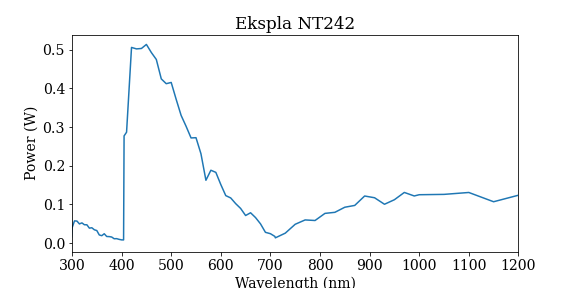
\includegraphics[width=\textwidth]{nt242_output.png}
    \caption{Expected Power output of NT242 Tunable Laser}
    \label{fig:laser_power}
\end{figure}


\subsection{White Light System}
plot of LEDs
Mechanical configuration
Optical model
Model output

\subsection{Projector}

\subsection{Monitoring systems}

We will want to measure precisely how much light from the laser is entering the CBP at a given wavelength so that we determine the exact fraction of that light that is captured by the LSST camera. In order to do that, we need to monitor the luminosity of the laser as it enters the integrating sphere as well as the spectral properties of the light. This data will be recorded for every measurement made with the CBP in such a way that it can be easily linked to the LSST camera image. 

\paragraph{\textbf{Photodiode}}

In order to monitor the exact amount of light injected into the CBP, we use a Hamamatsu S2281 Silicon Photodiode that has been precisely calibrated by NIST. 
This photodiode, which is mounted directly to the integrating sphere, has a sensitive area of 11 mm in diameter. It is read out by a Keithley 6517b electrometer. The electrometer can measure current, charge, resistance and voltage. Our uses of the CBP will likely use the charge and current modes. 

The electrometer can be read out as quickly as every 20 ms. There is a relationship between how long of an exposure you can take and the integration time. At the minimum integration time, you can take an exposure of $\sim$30 seconds. The data is saved in a fits file in the lfa with the elapsed time from the start of the exposure and the value measured. The range can be set to any value from X to Y. 

\paragraph{\textbf{Fiber Spectrograph}}

The spectral response of the injected light will be measured by a pair of fiber-fed spectrographs from Avantes SensLine, one for the blue wavelengths (range) and one for the red (range). These spectrographs will actually be housed in the central projection area in the center of the calibration screen. This is where light from the laser can be projected on the calibration screen. The fibers will be situated such that they will measure some fraction of reflected light within the projector box. When we want to measure the spectral response of the light, we will inject the fiber that runs to the calibration screen, take our measurement, and then send the laser light to the CBP. This assumes that the spectral response will not change from one output to another, which we will have to confirm.

The data from the spectrographs will be saved in a fits file in the lfa that will include the wavelength array and the counts measured by the spectrograph at that spacing.

\section{CBP}
The Rubin CBP was built by DFM Engineering. 
The design is essentially a Schmidt camera used in reverse. 
It includes a primary mirror of 33cm diameter, Schmidt Corrector and a 3-element Flat Field Corrector. 
It produces a beam with an aperture of 24.1 cm and a field of view of 4.1 degrees. 
The focal length of the CBP is 625mm, and with the LSST focal length at 10.1m, the magnification factor is 16. Therefore, a 100$\mu$m pinhole on the CBP would correspond to 1600 $\mu$m, or 160 pixels. 

\begin{table}[h!]
    \centering
    \begin{tabular}{|c|c|}
      \hline
       Aperture   & 24.1 cm \\
      \hline
      Focal Length   & 62.5 cm \\
      \hline
      Field of View & 4.1 degrees \\
      \hline
    \end{tabular}
    \caption{CBP Specifications}
    \label{tab:my_label}
\end{table}

The mount of the CBP allows movement in Azimuth and Elevation, with a swing diameter of 51.8". 
The locations are controlled by a Galil Digital Motor Controller (DMC) that is mounted on the azimuth housing. It controls the motors, reads the encoders, and interfaces to the control computer over ethernet. 
Additionally, the DMC controls the focus of the primary mirror and changes and rotates the masks. 
The azimuth and elevation stages are absolutely encoded with a Renishaw 26-bit on axis encoder. 


\begin{figure}[h]
    \centering
    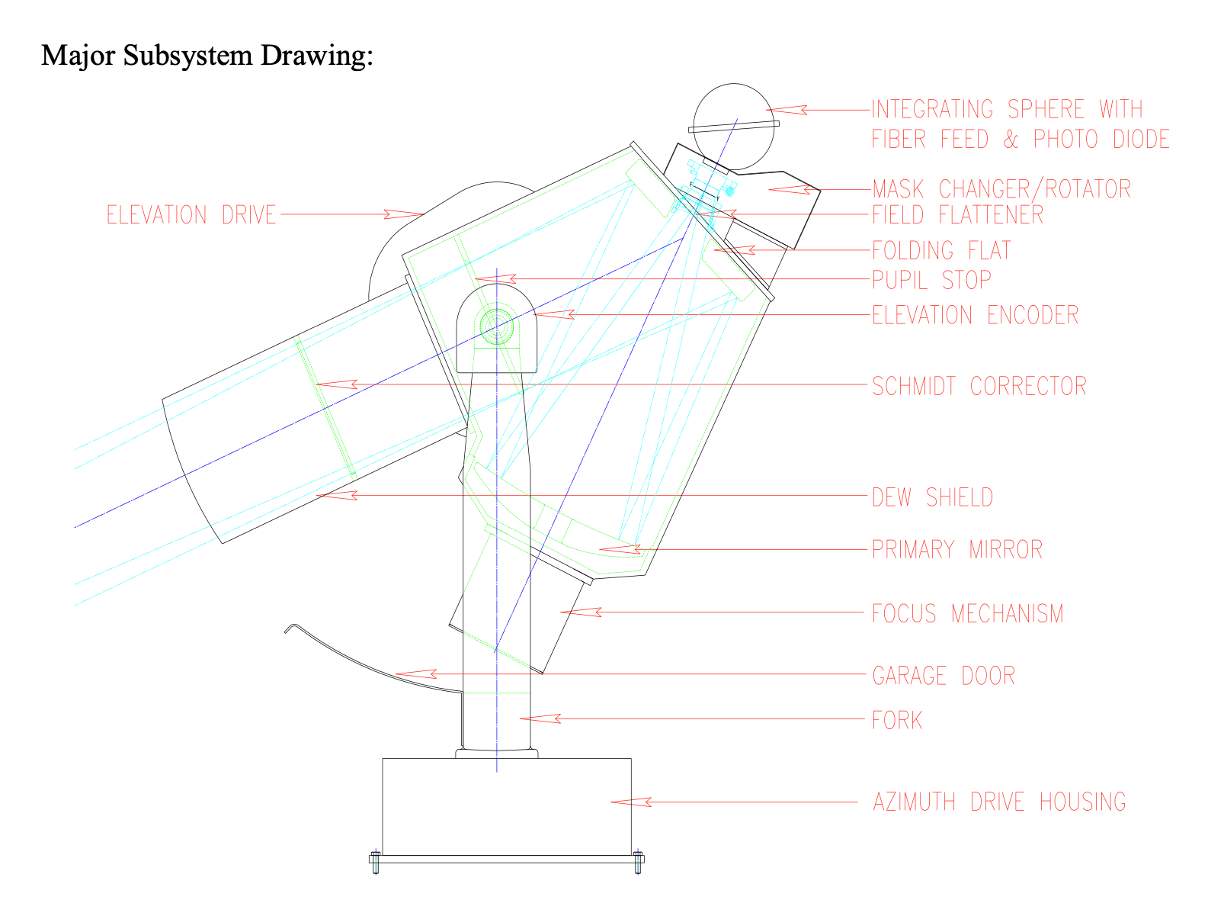
\includegraphics[width=\textwidth]{cbp_drawing.png}
    \caption{CBP Major subsystems}
    \label{fig:laser_power}
\end{figure}

At the focal plane sits the mask stage, which can hold 5 different masks. The masks can be rotated, driven by worm gears such that all masks are rotated on a common shaft by a single motor. The center mask stage is position encoded using a Renishaw absolute rotary encoder. The mask holder can hold masks with a diameter of 50 mm. Each mask will be laser etched into aluminium and are removable/interchangeable. 

The current Integrating Sphere installed on the CBP is a Labsphere 3P-GPS-060-SF. 
This integrating sphere has an interior diameter of 6 in. (152.4mm) and an exit port of 2.5 in. (63.5 mm), coated with spectraflect coating. 
In the exit port a photodiode will be mounted and it will be illuminated by an optical fiber.
The integrating sphere is held to the mask stage with standoffs. 
It sits $\sim 3$ in. from the focal plane/mask. 
Using \url{https://www.labsphere.com/wp-content/uploads/2021/09/Integrating-Sphere-Theory-and-Applications.pdf} as a guide to calculate the intensity of light exiting the integrating sphere by multiplying Ls by the flux incident on the integrating sphere.

\section{AuxTel/LATISS}

\section{Camera EOTest Data}

\section{On-Sky Data}
\subsection{Twilight Flats}
\subsection{Dense Dithered Star Fields}

\section{Plans Post-Year 1}
\subsection{Synethetic SED matched flats}
\subsection{Full CBP dataset}
% Include all the relevant bib files.
% https://lsst-texmf.lsst.io/lsstdoc.html#bibliographies
\section{References} \label{sec:bib}
\renewcommand{\refname}{} % Suppress default Bibliography section
\bibliography{local,lsst,lsst-dm,refs_ads,refs,books}

% Make sure lsst-texmf/bin/generateAcronyms.py is in your path
\appendix
\section{Calibration Products List}


\section{Acronyms} \label{sec:acronyms}
\addtocounter{table}{-1}
\begin{longtable}{p{0.145\textwidth}p{0.8\textwidth}}\hline
\textbf{Acronym} & \textbf{Description}  \\\hline

CBP & Collimated Beam Projector \\\hline
GPS & Global Positioning System \\\hline
ISR & Instrument Signal Removal \\\hline
LATISS & LSST Atmospheric Transmission Imager and Slitless Spectrograph \\\hline
LPM & LSST Project Management (Document Handle) \\\hline
LSE & LSST Systems Engineering (Document Handle) \\\hline
LSST & Legacy Survey of Space and Time (formerly Large Synoptic Survey Telescope) \\\hline
LTS & LSST Telescope and Site  (Document Handle) \\\hline
NIST & National Institute of Standards and Technology (USA) \\\hline
QE & quantum efficiency \\\hline
SE & System Engineering \\\hline
SED & Spectral Energy Distribution \\\hline
SF & Structure Function \\\hline
SRD & LSST Science Requirements; LPM-17 \\\hline
\end{longtable}


\begin{table}[h!]
    \begin{tabular}{|c|c|}
    Quantity & Product Description \\
    \hline \hline
    \textbf{Bias} & (combined) \\
    \hline
    \textbf{Dark} &  (combined) \\
    \hline
    \textbf{CTI} & what are these? \\  
    \hline
    \textbf{PTC} & Linearity + Gain \\
    \hline
    \textbf{C$_{i}$} & Crosstalk Matrix \\
    \hline
     & Defect masks \\
    \hline
    \textbf{BF} & Brighter-fatter kernels \\
    \hline
     & Fringe templates (zy) \\
    \hline
     & Lateral e-field templates \\
    \hline
    \textbf{QE$_{det}$} & Sensor QE \\ 
    \hline
    \textbf{R$_{mirror}$} & Mirror reflectivity (Silver x3) \\
    \hline
    \textbf{T$_{filter}$} & Filter transmission \\
    \hline
     & “White” light flats (ugrizy) \\ 
    \hline
    \textdf{T}(det, $\lambda$) & Transmission \\ 
    \hline
     & Dust flat (?) \\
    \hline
     & Twilight flats (ugrizy; combined) \\
    \hline
     & Sky flat (combined; ugrizy) \\
    \hline
     & Reference Flux Flat \\
    \hline
     & Dense dithered star field + lateral e-field (ugrizy) \\
    \hline
     & Survey observations \\
    \hline
    \end{tabular}
\end{table}

% \section{Acronyms} \label{sec:acronyms}
% \addtocounter{table}{-1}
\begin{longtable}{p{0.145\textwidth}p{0.8\textwidth}}\hline
\textbf{Acronym} & \textbf{Description}  \\\hline

CBP & Collimated Beam Projector \\\hline
GPS & Global Positioning System \\\hline
ISR & Instrument Signal Removal \\\hline
LATISS & LSST Atmospheric Transmission Imager and Slitless Spectrograph \\\hline
LPM & LSST Project Management (Document Handle) \\\hline
LSE & LSST Systems Engineering (Document Handle) \\\hline
LSST & Legacy Survey of Space and Time (formerly Large Synoptic Survey Telescope) \\\hline
LTS & LSST Telescope and Site  (Document Handle) \\\hline
NIST & National Institute of Standards and Technology (USA) \\\hline
QE & quantum efficiency \\\hline
SE & System Engineering \\\hline
SED & Spectral Energy Distribution \\\hline
SF & Structure Function \\\hline
SRD & LSST Science Requirements; LPM-17 \\\hline
\end{longtable}

% If you want glossary uncomment below -- comment out the two lines above
%\printglossaries





\end{document}
